\chapter{Funktionstest}
Nach der Implementierung des zuvor geschilderten Konzepts wurde ein Funktionstest durchgeführt.
Dazu werden zunächst die theoretischen Grenzen der Konfiguration getestet und danach die tatsächlichen Ausgabewerte mit den theoretischen verglichen.
Besonders interessant ist hierbei, in welchem Frequenzbereich der Generator zuverlässig funktioniert.

\section{theoretische Limitierungen}
Um den praktischen Nutzen des Funktionsgenerators einzuschätzen, werden die Grenzen der einstellbaren Frequenz, die Auflösung und der Spannungsbereich berechnet.
Für die Spannung ergeben sich diese Werte aus dem Datenblatt des eingesetzten DACs, dieser kann in einem Bereich von 0 bis 5,5 V eingesetzt werden, wobei die Referenzspannung 2,7 V nicht unterschreiten darf \cite{PmodDA2}.
Für den Betrieb auf dem Basys 3 Board läuft der Spannungsbereich von 0 bis 3,3 V, da hier die Ausgangsspannung des Boards der limitierende Faktor ist.
Nachfolgend werden noch der Frequenzbereich und die Auflösung bestimmt.

\subsection{Frequenzbereich}
Der Systemtakt $f_{sys}$ des Generators beträgt 100 MHz.
Der Frequenzbereich der Funktionen, die er ausgeben kann, reicht von ca. 0,0877 Hz bis zu ca. 735 kHz.
Die Frequenz $f_{count}$ ist die Frequenz mit der der interne Zähler der Funktionsbausteine hochzählt und beträgt ein 64tel des Systemtakts $f_{sys}$ (siehe \cref{test:theo:freq:fcount}).
Die minimale Frequenz $f_{min}$ errechnet sich aus dem maximalen Zählstand, der wiederum abhängig ist von seiner Bitbreite \code{clk\_width} (siehe \cref{test:theo:freq:fmin}).
Die maximale Frequenz ergibt sich aus dem Shannon'schen Abtasttheorem, nach dem die minimale Abtastfrequenz eines Signals doppelt so groß sein muss, wie die Frequenz des abgetasteten Signals \cite(blabla).
In diesem Fall entspricht die Abtastfrequenz $f_{count}$ und das abgetastete Signal dem Ausgangssignal, woraus folgt, dass das ausgehende Signal nur halb so groß sein kann, wie $f_{count}$ (siehe \cref{test:theo:freq:fmin}).

\begin{align}
  f_{count} &= \frac{f_{sys}}{68} \label{test:theo:freq:fcount}\\  
  f_{max} &= \frac{f_{count}}{2}  \label{test:theo:freq:fmax}\\ 
  f_{min} &= \frac{f_{count}}{2^{clk\_width} - 1} \label{test:theo:freq:fmin}
\end{align}

\subsection{Auflösung}
Die Auflösung des analogen Ausgangssignals hängt sowohl von der Geschwindigkeit ab, mit der das digitale Signal analogisiert werden kann, als auch von der maximalen Anzahl digital darstellbarer Werte.
Überschreitet die Frequenz des analogen Signals $f$ die Grenzfrequenz $f_{grenz}$, so fällt die Auflösung $R$ reziprok zu $f$ ab (siehe \cref{test:theo:res:plot}).
Oberhalb von $f_{grenz}$ ist die Auflösung durch die Bitbreite des ADCs begrenzt.
Da es sich um einen 12-Bit Wandler handelt, beträgt die Anzahl darstellbarer Werte und damit auch die höchste Auflösung $2^{12} = 4096$.
Diesen Wert nimmt die Auflösung an, wenn die Frequenz kleiner als $f_{grenz}$ ist (siehe \cref{test:theo:freq:fgrenz}).

\begin{align}
  R &= \begin{cases}
    4095               & f \leq f_{grenz}                      \\
    \frac{f_{count}}{f} & f > f_{grenz} = \frac{f_{count}}{4095} = 359 Hz
        \end{cases} \label{test:theo:freq:fgrenz}
\end{align}

Konkret bedeutet dass für den Funktionsgenerator, dass bei einer Amplitude von $U_{SS}=3,3V$ und einer Frequenz von $f=100kHz$, die Auflösung $4,54V^{-1}$ statt der maximalen Auflösung von $1241V^{-1}$ beträgt, das heißt, dass bei 100kHz 4,54 Werte statt 1241 Werte pro Volt gesampelt werden.

\begin{figure}[h] \centering
    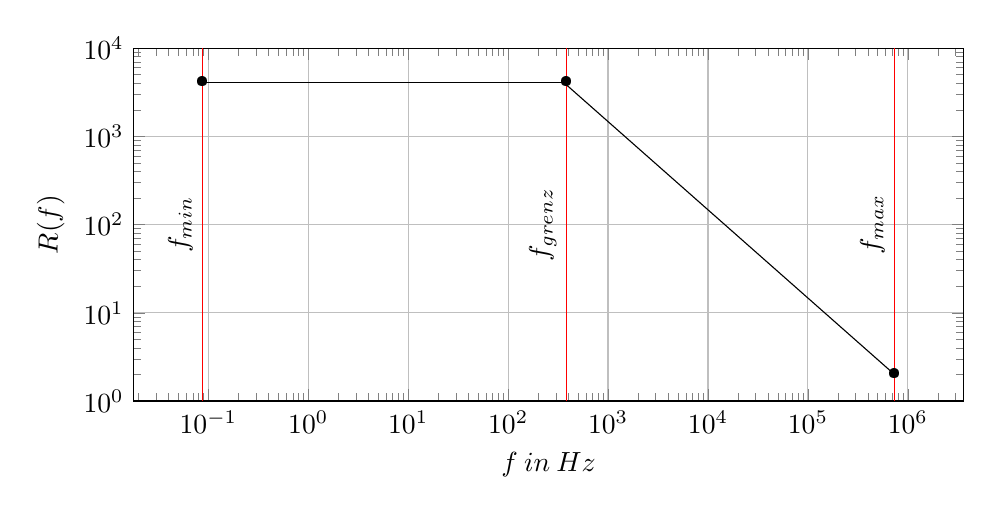
\begin{tikzpicture}
      \begin{loglogaxis}
        [xlabel=$f\:in\:Hz$,
        ylabel=$R(f)$,
        ymin=1,
        ymax=10000,,
        width=\textwidth,
        height=0.5\textwidth,
        grid=major]
        \addplot[color=black, domain=0.08765:359.12] {4095};
        \addplot[color=black, domain=359.12:735294] {100000000 / (68*\x)};
        % help lines and nodes:
        \addplot[color=red] coordinates{(381.12, 1)(381.12, 10000)};
        \node[above, rotate=90] at (381.12, 100) {$f_{grenz}$};
        \node at (381.12, 4095) {\textbullet};

        \addplot[color=red] coordinates{(0.08765, 1)(0.08765, 10000)};
        \node[above, rotate=90] at (0.08765, 100) {$f_{min}$};
        \node at (0.08765, 4095) {\textbullet};

        \addplot[color=red] coordinates{(735294, 1)(735294, 10000)};
        \node[above, rotate=90] at (735294, 100) {$f_{max}$};
        \node at (735294, 2) {\textbullet};
      \end{loglogaxis}
    \end{tikzpicture}
 \caption{Doppelt logarithmisches Diagramm der Auflösung $R(f)$ über den Frequenzbereich $f$. Die Auflösung bleibt konstant bei 4095 1/tick bis sie schließlich bei $f_{grenz}$ anfängt zu sinken.} \label{test:theo:res:plot}
\end{figure}

\section{reales Verhalten}
Nun soll das reale Verhalten des Funktionsgenerators untersucht werden.

\subsection{Versuchsaufbau}
Ein Foto des Versuchsaufbaus findet sich in \cref{test:real:setup:pic}.
Das digitale Oszilloskop Analog Discovery 2 von digilent wird dazu an einen Laptop angeschlossen, auf dem dann die Funktionsverläufe angezeigt werden.

\begin{figure}[h]
  \includegraphics[width=\textwidth]{testaufbau_fg}
  \caption{Versuchsaufbau zum Testen des Funktionsgenerators. Das Oszilloskopist mittels des Moduls Discovery BNC an den analog Ausgang des PmodDA2-Wandlers angeschlossen. Das Basys 3-Board wird über das angeschlossene USB Kabel mit Strom versorgt und per UART konfiguriert. Die vom Oszilloskop eingelesenen Daten werden an einen per USB angeschlossenen Laptop verschickt. Die LEDs auf dem Board zeigen den internen digitalen Funktionswert an.} \label{test:real:setup:pic}
\end{figure}

\subsection{Versuchsdurchführung}
Um zunächst die korrekte Ausgabe der Funktionsverläufe zu überprüfen, werden alle vier Verläufe nacheinander bei konstanter Frequenz $f=100Hz$ über die UART-Schnittstelle konfiguriert und die erfassten Signale dokumentiert.
Der eingestellte \analog{low} und \analog{high} Wert beträgt 0 bzw. 3,3 V.
Anschließend werden alle Funktionen der UART-Schnittstelle überprüft, indem der jeweilige Befehl mit einem dazu passenden Argument abgeschickt wird.
Schließlich wird noch der Frequenzbereich anhand der Zick-Zack-Funktion untersucht.
Dazu wird ein Wert knapp unterhalb von $f_{min}$ und ein Wert oberhalb von $f_{max}$ eingestellt.
Dazwischen wird, von 0.1 Hz aufwärts, mit jedem Schritt die eingestellte Frequenz mit 10 multipliziert.
Die Werte für \analog{low} und \analog{high} werden wieder auf 0 und 3,3 V gesetzt.
Auffäligkeiten im Funktionsverlauf werden festgehalten und die Daten werden dann noch im CSV Format für weitere Auswertungen abgespeichert.
Um die Frequenz der Zick-Zack Funktion zu messen, werden alle Datenpunkte mitAusgangsspannung $U < 0,5 V$ betrachtet.
Aus den Zeitkomponenten nahe beieinander liegender Punkte wird dann der Mittelwert gebildet.
Die Differenz zweier aufeinanderfolgender Mittelwerte kann als Näherung für die Zykluszeit $T$ betrachtet werden.
Aus der Zykluszeit wird dann die Frequenz des Signals $f = 1 / T$ berechnet.

\subsection{Ergebnis}
\begin{figure}[h] \centering
  {
    \pgfplotsset{
    no markers,
    grid=major,
    ymin=-0.2, ymax=3.5,
    scaled x ticks=false,
    ytick={0, 0.55, 1.1, 1.65, 2.2, 2.75, 3.3},
    xtick={-0.005, -0.0025, 0, 0.0025, 0.005},
    xticklabels={-5, -2.5, 0, 2.5, 5},
    width=0.5\textwidth}
  % constant
  \subfloat[][konstante Funktion]{ 
    \begin{tikzpicture}
      \begin{axis}[ylabel=$U(t)$ in V]
        \addplot table [x=Time (s), y=Channel 2 (V), col sep=comma, row sep=newline] {test/const100Hz_small.csv};
      \end{axis}
    \end{tikzpicture}
    \label{test:real:res:plot:const}
  } 
  % square
  \subfloat[][Rechteckfunktion]{
    \begin{tikzpicture}
      \begin{axis}
        \addplot table [x=Time (s), y=Channel 2 (V), col sep=comma, row sep=newline] {test/square100Hz_small.csv};
      \end{axis}
    \end{tikzpicture}
    \label{test:real:res:plot:square}
  } 

  % zigzag 
  \subfloat[][Zick-Zack-Funktion]{
    \begin{tikzpicture}
      \begin{axis}[ylabel=$U(t)$ in V, xlabel=$t$ in ms]
        \addplot table [x=Time (s), y=Channel 2 (V), col sep=comma, row sep=newline] {test/zigzag100Hz_small.csv};
      \end{axis}
    \end{tikzpicture}
    \label{test:real:res:plot:zigzag}
  }
  % ramp
  \subfloat[][Rampenfunktion]{
    \begin{tikzpicture}
      \begin{axis}[xlabel=$t$ in ms]
        \addplot table [x=Time (s), y=Channel 2 (V), col sep=comma, row sep=newline] {test/ramp100Hz_small.csv};
      \end{axis}
    \end{tikzpicture}
    \label{test:real:res:plot:ramp}
  }
}
  \caption{Die Ergebnisse des Versuchs bei $f=100Hz$. Besonders bei der konstanten Funktion und bei der Rechteckfunktion kann man ein leichtes Rauschen erkennen. An der Rechteckfunktion kann man auch sehen, dass der \analog{low} Wert dauerhaft unter 0 V liegt.} \label{test:real:res:plot}
\end{figure}


Die Funktionsverläufe bei $f = 100Hz$ ergaben sich auf den ersten Blick wie erwartet.
Ihre Frequenz wurde mit dem Cursor-Tool der Oszilloskop Software gemessen und ergab ca. 100 Hz.
Jedoch fiel auf, dass \analog{low} und \analog{high} nicht genau 0 bzw. 3,3 V betrugen.
Der Mittelwert des konstanten Signals betrug $\overline{U}_{c}=3,24 V$, beim Rechtecksignal lag der tiefste Wert bei $U_{sl} = -0,11 V$ und der höchste bei $U_{sh} = 3,25 V$, beim Zick-Zack-Signal waren es $U_{zzl} = -0,06 V$ und $U_{zzh} = 3,26 V$ und beim Rampensignal $U_{rl} = -0,1 V$ und $U_{rh} = 3,24 V$.
Jeweils ein Zyklus pro Funktion ist in \cref{test:real:res:plot} dargestellt.\\
Der Generator ließ sich problemlos per UART konfigurieren.
Alle eingegebenen Befehle führten zu der erwarteten Ausgabe am analogen Ausgang.\\
Beim Abtasten der Frequenz  ergab sich bei Unterschreiten von $f_{min}$ ($f = 0.08Hz$) eine wesentlich höhere Frequenz von 20,5 Hz. 
Im niedrigen Frequenzbereich konnten nur geringe Abweichungen von der eingestellten Frequenz gemessen werden.
Je näher $f$ jedoch $f_{max}$ kam, desto stärker wich die gemessene von der eingestellten Frequenz ab.
Außerdem wurde das Signal immer undeutlicher, bis es schließlich bei $f > f_{max}$ so unkenntlich war, dass die Frequenz nicht mehr bestimmt wurde.
Alle anderen Messergebnisse finden sich in \cref{test:real:res:ftab}.

\begin{table}[h]
  \begin{tabular}[h]{|l|r|r|r|r|r|r|r|r|r|r|}
    \hline
    $f_{soll}$ in Hz & 0,08 & 0,1 & 1 & 10 & 100 & $10^3$ & $10^4$ & $10^5$ & $3,5 \cdot 10^5$ & $10^6$\\ \hline
    $f_{ist}$ in Hz & 20,5 & 0,100 & 1,01& 10,1 & 101 & 999 & $10^4$ & $9,81 \cdot 10^4$ & $2,94 \cdot 10⁵$ & - \\ \hline
  \end{tabular}
  \caption{Diese Tabelle stellt die eingestellten Frequenzen $f_{soll}$ den gemessenen Frequenzen $f_{ist}$ gegenüber. Für $f_{soll} = 10^6$ konnte die Frequenz nicht bestimmt werden.} \label{test:real:res:ftab}
\end{table}

% auswertung
\subsection{Auswertung}


